%\documentclass[oneside,12pt]{article}
\documentclass[oneside]{article}
%\documentclass[12pt]{report}
%\documentclass[12pt,a4paper,english,danish]{report}

\usepackage{hyperref}
\usepackage{multirow}
\usepackage[pdftex]{graphicx}
\usepackage{epstopdf}
%\usepackage{epsfig}
\usepackage{listings}
\usepackage{subfigure}
\usepackage{url}
\usepackage{amsmath}
\usepackage{amssymb}
\usepackage{enumitem}
%\usepackage{enumerate}
%\usepackage[latin1]{inputenc}
%\usepackage{url}

\usepackage{color}                       % colors
\definecolor{lightgrey}{rgb}{0.9,0.9,0.9} % color values Red, Green, Blue
\definecolor{lightred}{rgb}{0.9,0.7,0.7} % color values Red, Green, Blue
\definecolor{lightgreen}{rgb}{0.7,0.9,0.7} % color values Red, Green, Blue
\definecolor{lightblue}{rgb}{0.5,0.7,0.9} % color values Red, Green, Blue
\definecolor{blue}{rgb}{0.0,0.43,0.72}
\definecolor{red}{rgb}{0.6,0.0,0.0}


\lstset{keywordstyle=\color{blue}\bfseries}

\lstset{ %
language=C,                % choose the language of the code
basicstyle=\footnotesize\ttfamily,       % the size of the fonts that are used for the code
numbers=none,                   % where to put the line-numbers
numberstyle=\footnotesize,      % the size of the fonts that are used for the line-numbers
stepnumber=2,                   % the step between two line-numbers. If it's 1 each line will be numbered
numbersep=5pt,                  % how far the line-numbers are from the code
backgroundcolor=\color{lightgrey},  % choose the background color. You must add \usepackage{color}
showspaces=false,               % show spaces adding particular underscores
showstringspaces=false,         % underline spaces within strings
showtabs=false,                 % show tabs within strings adding particular underscores
frame=single,                   % adds a frame around the code
tabsize=2,                      % sets default tabsize to 2 spaces
captionpos=b,                   % sets the caption-position to bottom
breaklines=true,                % sets automatic line breaking
breakatwhitespace=false,        % sets if automatic breaks should only happen at whitespace
escapeinside={\%*}{*)}          % if you want to add a comment within your code
}



\newcommand{\reff}[1]{(\ref{#1})}
\newcommand{\captionx}[1]{\centering\begin{minipage}{.80\textwidth}\caption{#1}\end{minipage}}

\DeclareMathOperator*{\mle}{arg\; max} 


\begin{document}

\title{Darknet \& Yolo3}
\author{Joe Hoeller
}
\maketitle

\begin{abstract}



\end{abstract}
%\clearpage


%\tableofcontents

%\clearpage
\section{Neural Network, Data Engineering and Hyper-Parameter Choices}
\subsection{Neural Network Choice and Justification}
Yolov3 with Spatial Pooling (SPP) Blocks was chosen because SPP block extract more relevant features to operate on. This results in increased knowledge of classes, and the 52 x 52 layer in Yolov3 detects the smaller objects quite well, this is useful for objects in the distance or down the street in FLIR images. Note that in the CNN architecture there is not a softmaxing of class scores. This is also useful if we wanted to do transfer learning later on, and train classes like taxi, truck or electric vehicle.

Yolov3-SPP also has residual skip connections, and upsampling, but the most salient feature of v3 is that it makes detections at three different scales. In YOLO v3, the detection is done by applying 1 x 1 detection kernels on feature maps of three different sizes at three different places in the network.

\begin{figure}
\centering
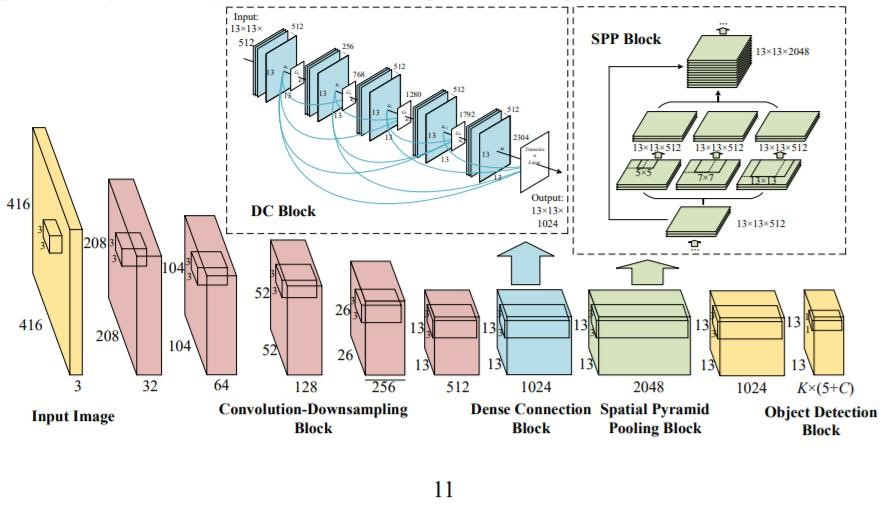
\includegraphics[width=0.8\linewidth]{images/spp-f1}
\caption{Yolo3-SPP}
\label{fig:spp-f1}
\end{figure}
To understand and visualize SPP Blocks a bit more, in \textsf{yolov3-spp.cfg}, they use 3 different size max pooling to the same image by using [route]. After that, they collect created feature map as called "fixed-length representation" regardless of image size and scale, as To understand and visualize SPP Blocks a bit more, in \textsf{yolov3-spp.cfg}, they use 3 different size max pooling to the same image by using [route]. After that, they collect created feature map as called "fixed-length representation" regardless of image size and scale, as stated above. More on SPP can be found in this research paper here \cite{He2014}.

\begin{figure}
\centering
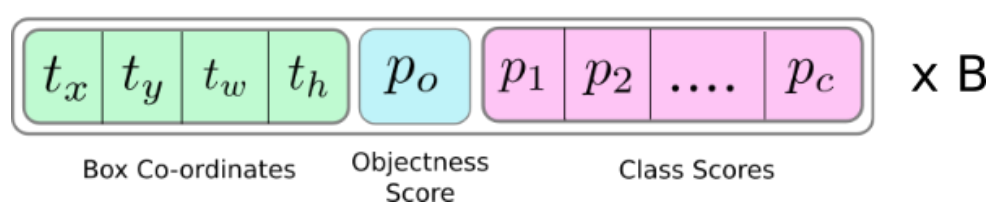
\includegraphics[width=0.7\linewidth]{images/spp-f2}
\caption{}
\label{fig:spp-f2}
\end{figure}


\begin{figure}
\centering
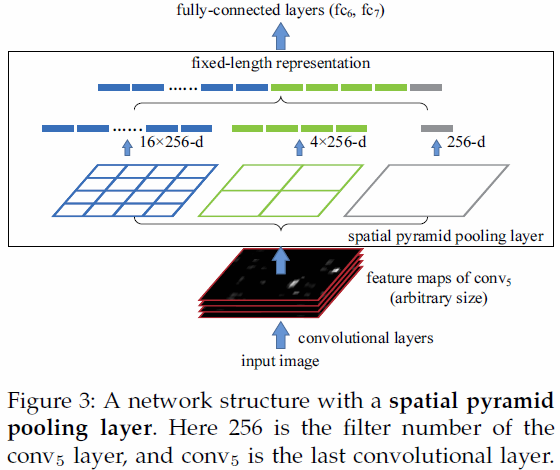
\includegraphics[width=0.7\linewidth]{images/spp-f3}
\caption{}
\label{fig:spp-f3}
\end{figure}

After I researched the features of the of Yolov3 architecture, it led me to SPP blocks. Which then led me to choosing a Darknet port of Yolov3: I used Ultralytics Yolov3. 

GitHub link here: \href{https://github.com/ultralytics/yolov3}{Ultralytics yolov3}.

\subsection{Data Engineering for FLIR Dataset: GIGO or...?}
After reading the limited documentation and making two pull requests for them to fix bugs, on Ultralytics (which they did), I ended up creating my own COCO to Darknet Annotation conversion tool, called Dark Chocolate, GitHub link here: https://github.com/joehoeller/Dark-Chocolate.

Why did I do that? To do some “maths” that baked in error correction during the conversion, so when the images were ran through the neural network, it produced a more precise IoU score, which ultimately boosted the mAP.


For example, when I converted the data set with this conversion tool already available, \href{https://github.com/enesozi/object-detection/blob/master/convert\_coco_yolo.py}{convert\_coco\_yolo.py}, I got a different result.\

Whereas, when I used the tool I made, “Dark Chocolate”, it computed the precision and values ever so slightly different, which made a very positive impact on the end result.

(For example, 0.4609375 versus 0.460938 and 0.7015625 versus 0.701562,
and so forth):

\newpage
\begin{figure}
\centering
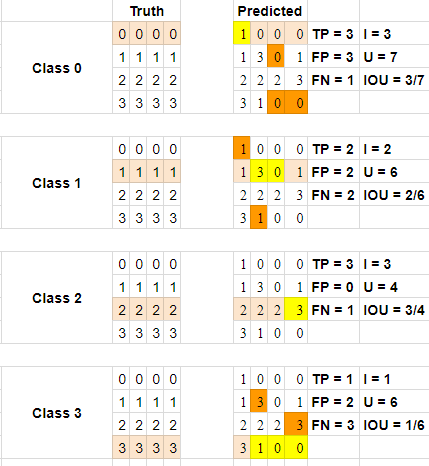
\includegraphics[width=0.7\linewidth]{images/confusion-f1}
\caption{Improved IOU Calculation from Annotated Inputs}
\label{fig:confusion-f1}
\end{figure}
To the right, the left side is our ground
truth, while the right side contains our predictions. The highlighted cells on the
left side note which class we are looking
at for statistics on the right side. The
highlights on the right side note true
positives in a cream color, false positives
in orange, and false negatives in yellow
(note that all others are true negatives -
they are predicted as this individual class,
and should not be based on the ground truth).
For Class 0, only the top row of the 4x4 matrix should be predicted as zeros. This is a rather simplified version of a real ground truth - in reality, the zeros could be anywhere in the matrix. On the right side, we see 1,0,0,0, meaning the first is a false negative, but the other three are true positives (aka 3 for Intersection as well). From there, we need to find anywhere else where zero was falsely predicted, and we note that happens once on the second row, and twice on the fourth row, for a total of three false positives.

 To get the Union, we add up TP (3), FP (3) and FN (1) to get seven. The IOU for this class,  
 therefore, is 3/7.

 If we do this for all the classes and average the IOUs, we get:
       Mean IOU = [(3/7) + (2/6) + (3/4) + (1/6)] / 4 = 0.420

\subsection{Hyper-parameter Choices}
I kept the yolov3-spp.cfg in it’s default configuration, sans the param’s at the end and beginning of each of the three Yolo layers, which were classes and filters. I used the following calculation to determine the number of filters for each layer, based on number of classes:

(4 + 1 + 17) * 3 = 66
17 classes, 66 filters
\begin{figure}
\centering
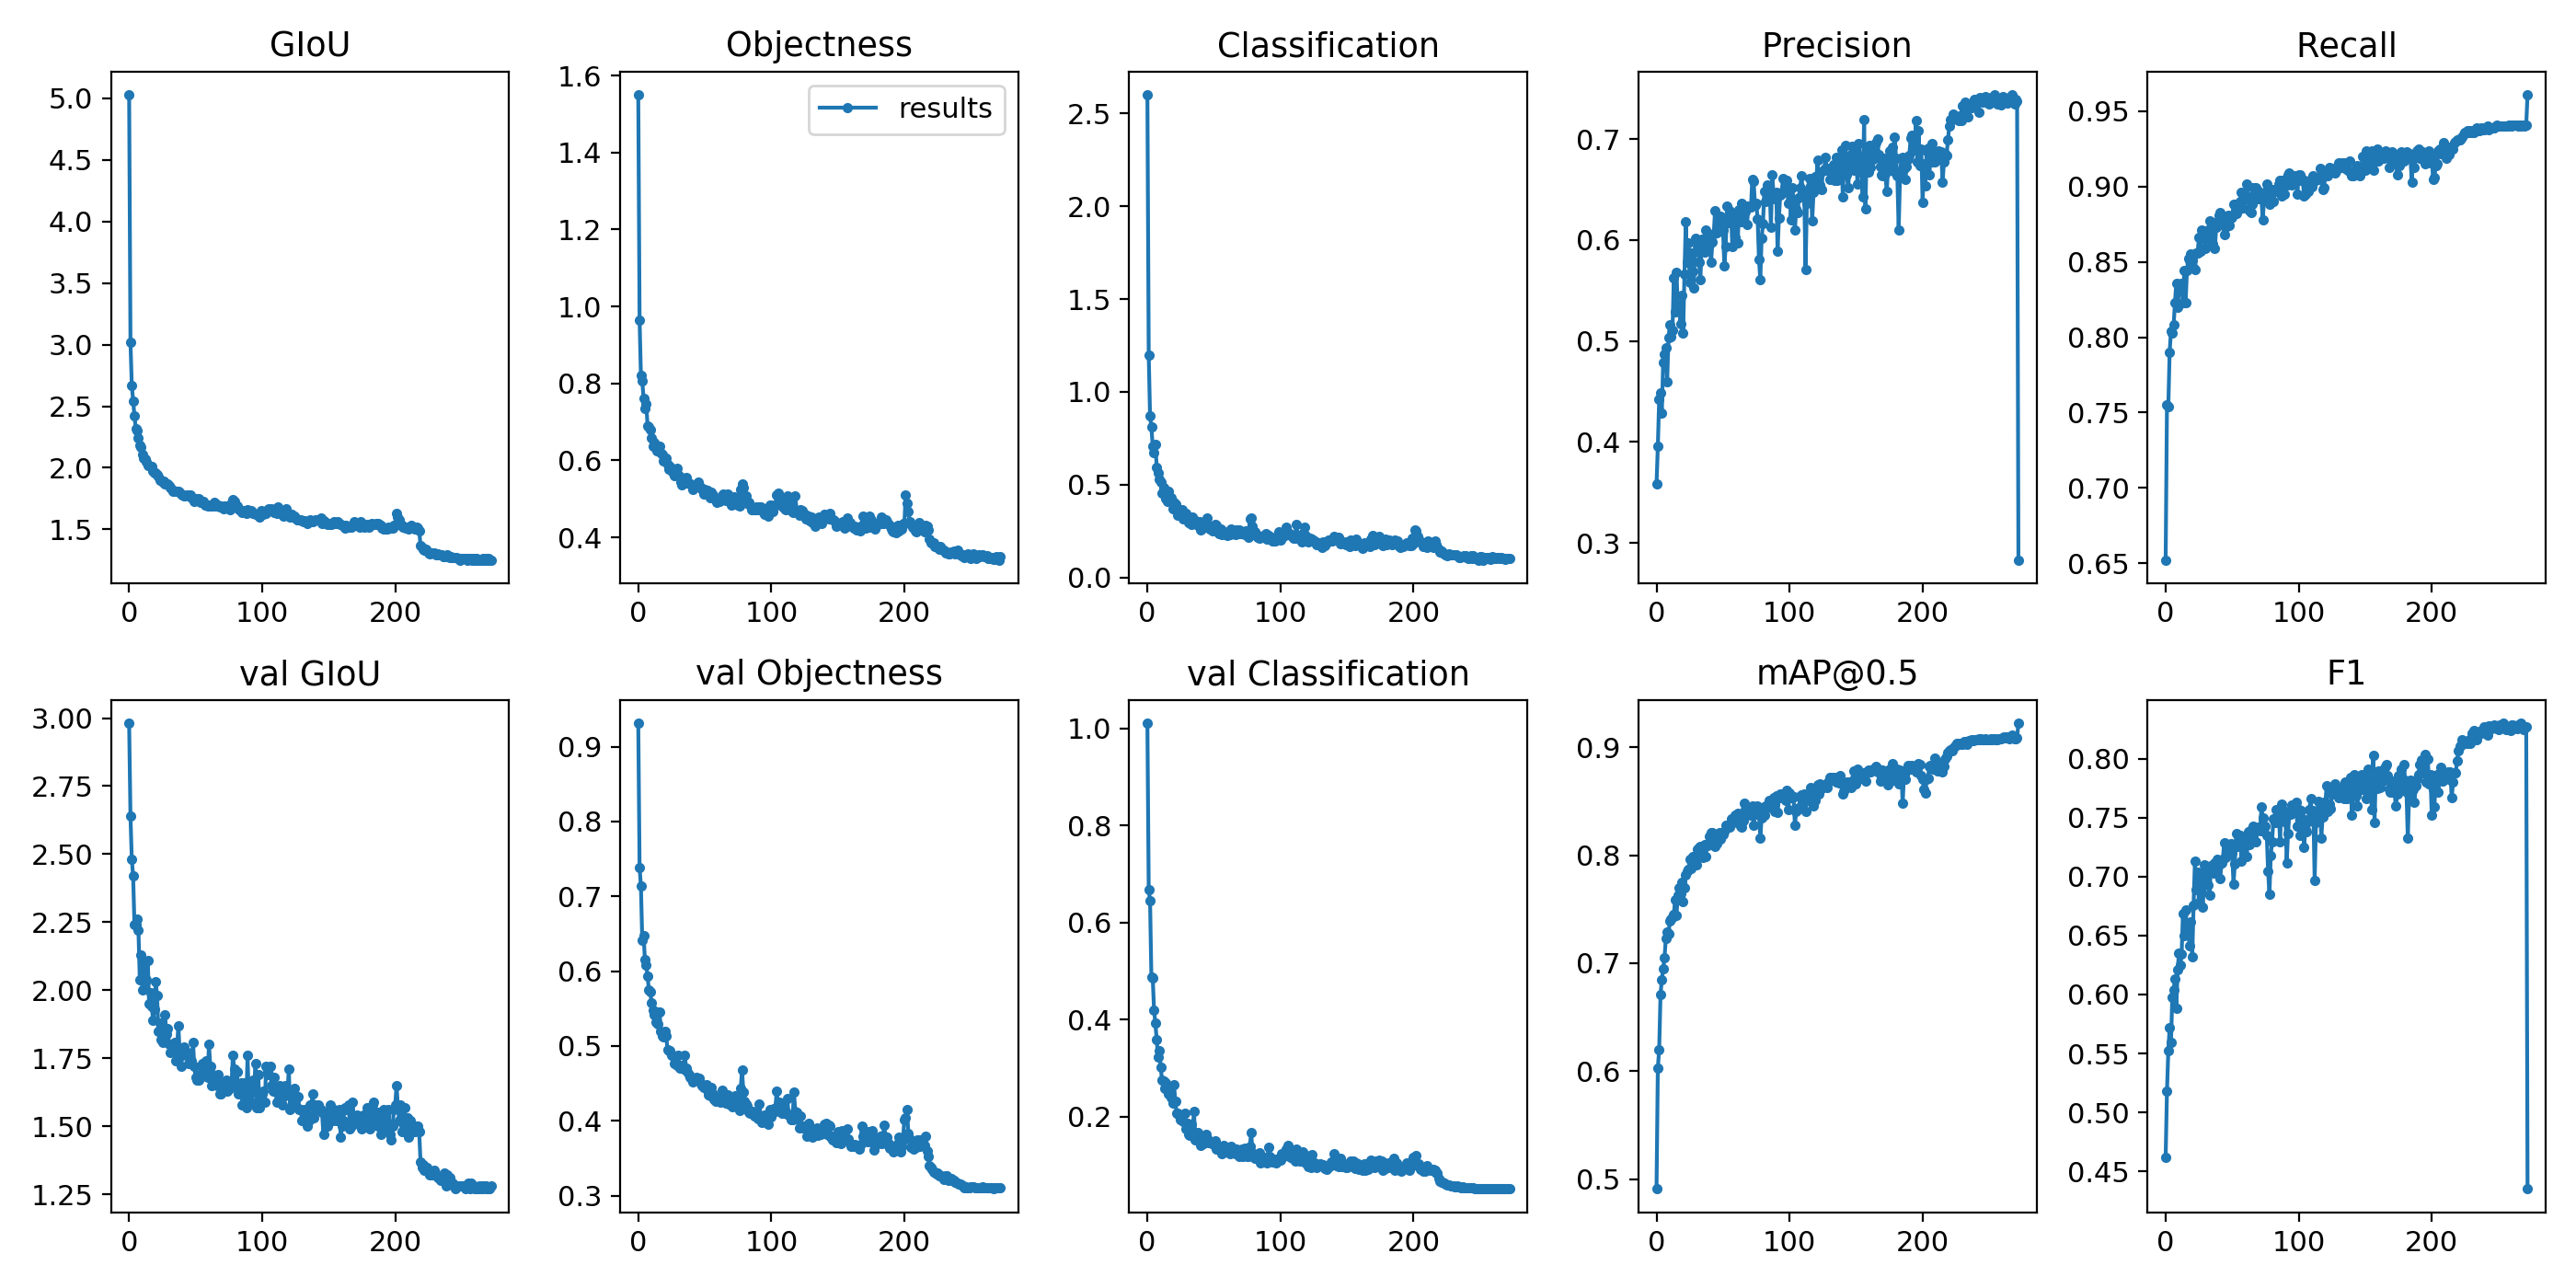
\includegraphics[width=0.7\linewidth]{images/results-f1}
\caption{After 272 training epochs  mAP: 0.961, Recall 0.922, F1: 0.857}
\label{fig:results-f1}
\end{figure}

\begin{figure}
\centering
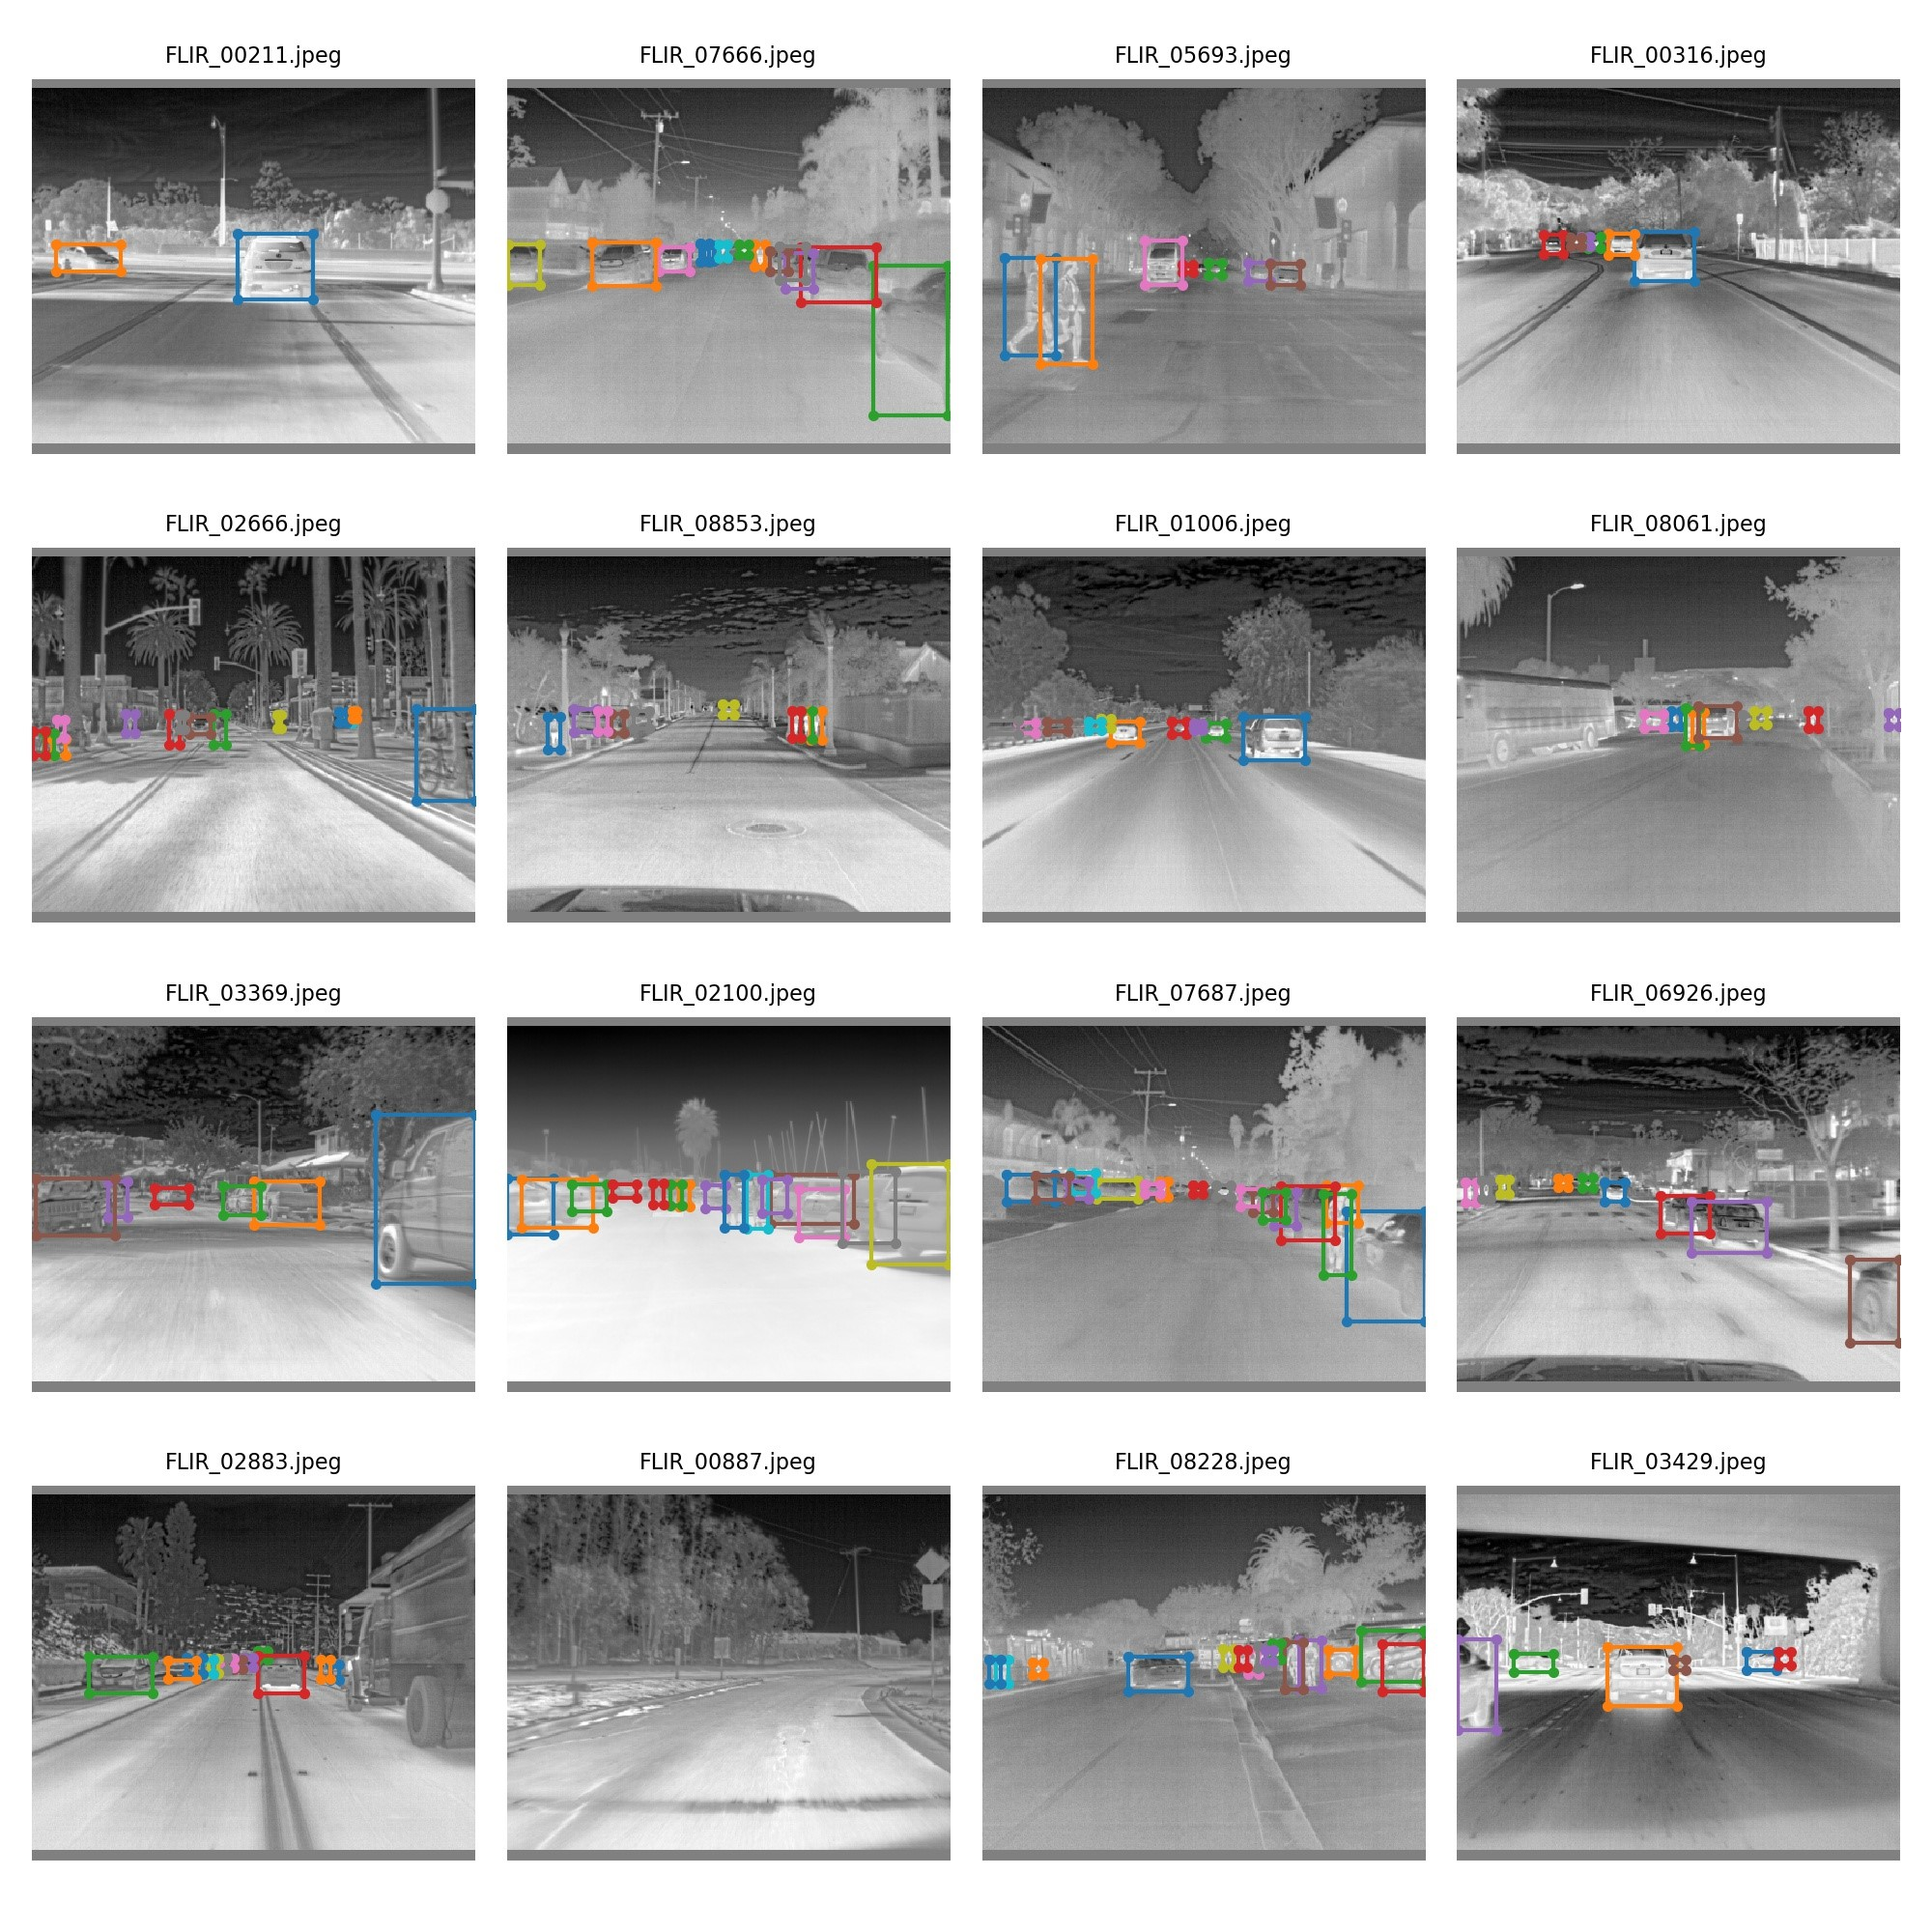
\includegraphics[width=0.7\linewidth]{images/results-f2}
\caption{See cars 0.57, 1.00, 0.99, 0.86, mostly obstructed and far off in distance and it still detected them:
}
\label{fig:results-f2}
\end{figure}
As stated above, Yolov3-spp doesn't softmax classes, SPP blocks extract more and better features, as well as Yolov3’s 52 x 52 layer detects the smaller objects better. This combination aided in detecting objects that were down the street and far off in the distance, or obstructed and/or mostly hidden from foreground objects,
as shown in a few samples below \ref{fig:results-f2}:

\begin{figure}
\centering
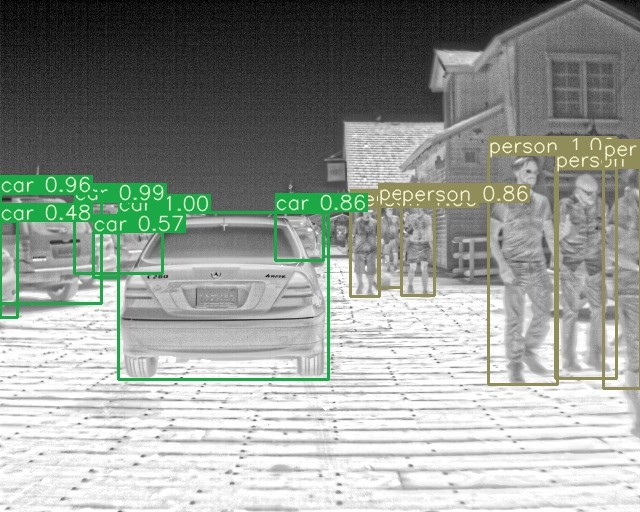
\includegraphics[width=0.7\linewidth]{images/results-f3}
\caption{See lots of people in distance standing in front of one another}
\label{fig:results-f3}
\end{figure}

\begin{figure}
\centering
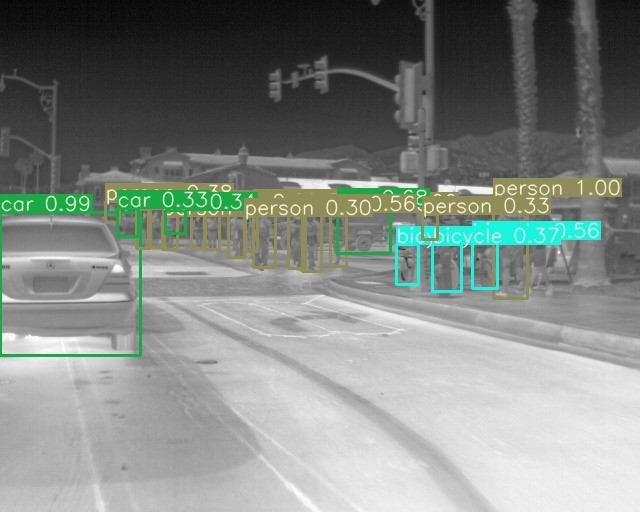
\includegraphics[width=0.7\linewidth]{images/results-f4}
\caption{}
\label{fig:results-f4}
\end{figure}

\begin{figure}
\centering
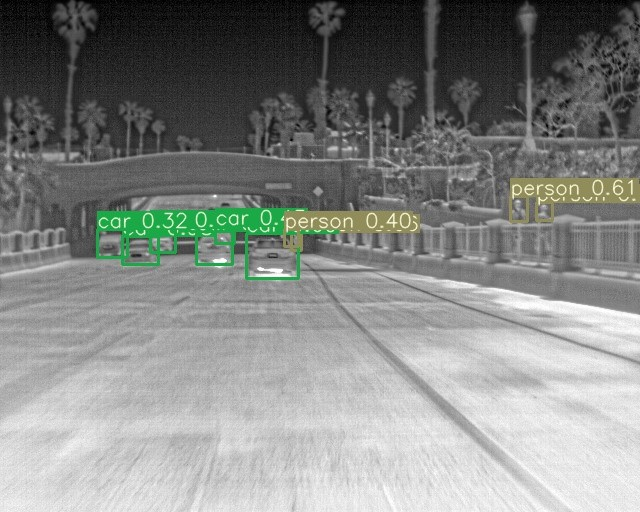
\includegraphics[width=0.7\linewidth]{images/results-f5}
\caption{ Detected half of a person obstructed by railing}
\label{fig:results-f5}
\end{figure}

\begin{figure}
\centering
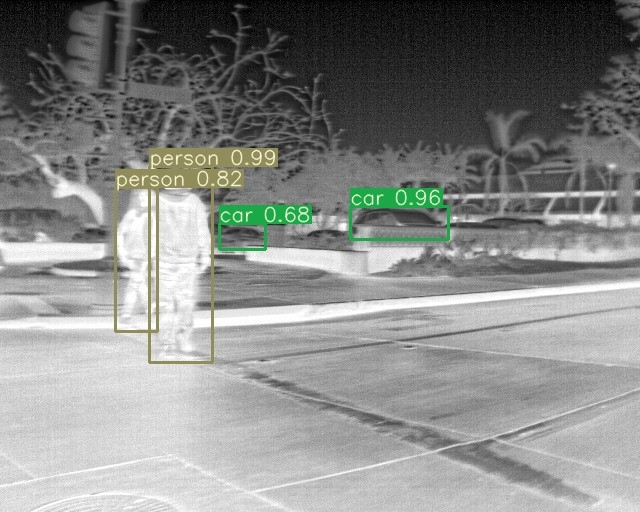
\includegraphics[width=0.7\linewidth]{images/results-f6}
\caption{Cars mostly obstructed by wall, especially car 0.68 in parking lot}
\label{fig:results-f6}
\end{figure}

\newpage
\section{Conclusion}

\section{Remarks}


\vspace{24pt} \noindent\textbf{Acknowledgments.}{\small \quad
Finally, thank you to my friends for the support during this report.
}



\bibliographystyle{alpha}
\small{\bibliography{my-refs}}




%\appendix

\end{document}